\documentclass{abntpuc}

\usepackage{amsmath} 
\usepackage{graphicx}
\usepackage{titlesec}
\usepackage{hyperref}
\usepackage{nameref}

\titleformat{\chapter}[display]
  {\normalfont\Large\bfseries}
  {\chaptername\ \thechapter}
  {10pt}
  {\Large}

\titleformat{\section}
  {\normalfont\LARGE\bfseries}
  {\thesection\hspace{1em}}
  {1em}
  {}
 
\universidade   {Pontifícia Universidade Católica de São Paulo}
\faculdade      {Faculdade de Estudos Interdisciplinares}
\departamento   {Departamento de Ciência de Dados e Inteligência Artificial}
\curso          {Ciência de Dados e Inteligência Artificial}
\grau           {Bacharel}
\author         {Gabriel Machado \\ João Pedro Garcia \\ Matheus Lopes \\ Miguel Battendieri \\ Pedro Vendrametto}
\trabalho       {Relatório Final do Projeto de Predição de Fraude em Dados de Cartão de Crédito}
\titulo         {Projeto de Predição de Fraude em Dados de Cartão de Crédito}
\cidade         {São Paulo}
\orientador     {Prof. Rooney Albuquerque}
\ano            {2024}
\datacompleta   {30 de setembro de 2024}

\palavraschave  {Modelo ABNT}{PUC-SP}{Iniciação Científica}{Relatório Final}

\preambulo      {Projeto de Predição de Fraude em Dados de Cartão de Crédito (Pontifícia Universidade Católica de São Paulo)}


\begin{document}

\capa

\folharosto

\tableofcontents

\chapter{Introdução}

De maneira geral, podemos nos referir à incapacidade de um cliente de pagar, inadimplência em um pagamento ou falência pessoal como potenciais problemas de não pagamento. No entanto, cada um desses cenários resulta de diferentes circunstâncias, como perda de emprego, problemas de saúde ou incapacidade de trabalhar. Às vezes, é um ato deliberado, quando o cliente sabe que não tem mais condições de usar o cartão de crédito, mas continua usando até que o banco cancele o cartão, caracterizando fraude, o que é difícil de prever e um grande problema para os credores.

Para resolver esse problema, as empresas de cartão de crédito tentam prever possíveis inadimplências ou avaliar a probabilidade de risco em um pagamento antecipadamente. Quanto mais cedo as contas potenciais de inadimplência forem detectadas, menores serão as perdas para os credores. Por isso, uma abordagem eficaz para prever inadimplência potencial é crucial para permitir que os credores tomem ações preventivas e também possam ajudar o cliente a evitar falências, minimizando as perdas.

Analisar milhões de transações e fazer previsões com base nisso é demorado, consome muitos recursos e pode ser suscetível a erros devido a variáveis dinâmicas (como limite de saldo, renda, condições econômicas, etc.). Portanto, há uma necessidade de abordagens otimizadas que possam lidar com essas restrições.

A regressão logística é uma técnica estatística usada para modelar a probabilidade de um evento binário. É amplamente utilizada em estatística e aprendizado de máquina para classificação binária.

\section{Problema de Pesquisa}

Como prever a inadimplência de clientes de cartão de crédito, utilizando técnicas de aprendizado de máquina, a fim de minimizar os riscos financeiros de uma instituição?

\section{Objetivo Geral}

Desenvolver um modelo de predição de inadimplência em cartões de crédito, utilizando como base um conjunto de dados de clientes, com o objetivo de auxiliar na tomada de decisão e na gestão de riscos de crédito.

\section{Objetivos Específicos}

\begin{itemize}
    \item Realizar uma análise exploratória dos dados para identificar padrões e características relevantes para a predição da inadimplência.
    \item Preparar os dados para a modelagem, incluindo tratamento de dados faltantes, codificação de variáveis categóricas e divisão do conjunto de dados em treinamento e teste.
    \item Treinar e avaliar um modelo de regressão logística para prever a probabilidade de inadimplência de um cliente.
    \item Analisar a performance do modelo através da matriz de confusão e outras métricas relevantes.
\end{itemize}

\section{Referencial Teórico}

A inadimplência de crédito é um problema recorrente no setor financeiro e tem sido objeto de diversas pesquisas. Autores como Thomas M. Wilson e Thomas C. Wilson destacam a importância da análise de dados e do uso de modelos preditivos para a gestão de riscos de crédito em um ambiente cada vez mais complexo.
A regressão logística, técnica popularizada por David Cox, continua sendo uma ferramenta fundamental, mas tem sido complementada por técnicas mais avançadas de machine learning, como redes neurais e random forests, como explorado por Breiman (2001).

\begin{quote}
    "A modelagem de crédito é uma ferramenta essencial para as instituições financeiras, permitindo a avaliação do risco de crédito e a tomada de decisões mais assertivas." 
\end{quote}
\rightline{Wilson T.M.}


\section{Metodologia}

Nesta seção, detalhamos as etapas seguidas para a realização deste estudo, desde a coleta de dados até a avaliação do modelo de predição de inadimplência.

\subsection{Coleta de Dados}
Os dados utilizados neste estudo foram baixados via Kaggle e gentilmente fornecidos pela University of California.

Agradecimentos: Agradecemos à UCI Machine Learning Repository pela disponibilização do conjunto de dados original, que pode ser acessado em: \\
\hypertarget{dataset_uci}{\url{https://archive.ics.uci.edu/ml/datasets/default+of+credit+card+clients}}


Referência: Lichman, M. (2013). UCI Machine Learning Repository [\hypertarget{uci}{\url{http://archive.ics.uci.edu/ml}}]. Irvine, CA: University of California, School of Information and Computer Science.

O conjunto de dados compreende informações de cerca de 30 mil clientes, incluindo variáveis como:

\begin{itemize}
    \item Demográficas: idade, sexo, estado civil, escolaridade.
    \item Financeiras: limite de crédito, histórico de pagamentos, saldo devedor, valor das faturas.
    \item Comportamentais: número de vezes que o limite foi excedido, quantidade de compras parceladas.
\end{itemize}

\subsection{Análise Exploratória de Dados}
A análise exploratória dos dados foi realizada utilizando a biblioteca Pandas do Python. Foram calculadas estatísticas descritivas (média, mediana, desvio padrão, mínimo, máximo) para as variáveis numéricas e realizadas análises de frequência para as variáveis categóricas.
Além disso, foram gerados gráficos como histogramas, boxplots e gráficos de dispersão para visualizar a distribuição dos dados e identificar possíveis relações entre as variáveis.

\subsection{Preparação dos Dados}
Antes de aplicar o modelo de regressão logística, os dados foram pré-processados da seguinte forma:
\begin{itemize}
    \item Tratamento de dados dúbios: Usando a descrição dada que fornece o que significam cada uma das variáveis categóricas que nos foram dadas nós manipulamos a exclusão das minoritárias para facilitar a boa performance do modelo, isso inclui também a técnica de conurbar aquelas categorizações que são semelhantes na nossa interpretação como grupo.
    \item Codificação de variáveis categóricas: Variáveis categóricas já foram codificadas utilizando a técnica de one-hot encoding (0-1) e também label.
    \item Normalização: Os dados numéricos foram normalizados utilizando a função StandardScaler para garantir que todas as variáveis tenham a mesma escala.
\end{itemize}

\subsection{Modelagem}
Um modelo de regressão logística foi utilizado para prever a probabilidade de inadimplência. A biblioteca scikit-learn do Python foi utilizada para implementar o modelo. As seguintes etapas foram realizadas:

\begin{itemize}
    \item Seleção de variáveis: As variáveis independentes mais relevantes para a predição da inadimplência foram selecionadas utilizando técnicas de seleção de características, como a análise do Score que correlaciona os vínculos entre as colunas.
    \item Treinamento do modelo: O modelo de regressão logística foi treinado utilizando o conjunto de dados de treinamento, ajustando os parâmetros do modelo para minimizar a função de perda.
    \item Validação do modelo: A performance do modelo foi avaliada utilizando o conjunto de dados de teste, calculando métricas como a matriz de confusão, acurácia, precisão, recall e F1-score.
\end{itemize}

\subsection{Avaliação do Modelo}
A matriz de confusão foi utilizada para avaliar a performance do modelo, permitindo visualizar os casos de acertos e erros nas predições. Além disso, foram calculadas as seguintes métricas:

\begin{itemize}
    \item \textbf{Acurácia}: Proporção de exemplos corretamente classificados (tanto positivos quanto negativos). A fórmula é dada por:
    \[
    \text{Acurácia} = \frac{TP + TN}{TP + TN + FP + FN}
    \]
    onde:
    \begin{itemize}
        \item \(TP\) (True Positives) são os exemplos positivos corretamente classificados;
        \item \(TN\) (True Negatives) são os exemplos negativos corretamente classificados;
        \item \(FP\) (False Positives) são os exemplos negativos incorretamente classificados como positivos;
        \item \(FN\) (False Negatives) são os exemplos positivos incorretamente classificados como negativos.
    \end{itemize}

    \item \textbf{Precisão}: Proporção de exemplos classificados como positivos que realmente são positivos. A fórmula é dada por:
    \[
    \text{Precisão} = \frac{TP}{TP + FP}
    \]
    
    \item \textbf{Recall (Sensibilidade)}: Proporção de exemplos positivos corretamente classificados entre todos os exemplos realmente positivos. A fórmula é:
    \[
    \text{Recall} = \frac{TP}{TP + FN}
    \]
    
    \item \textbf{F1-Score}: Média harmônica entre a precisão e o recall, utilizada para balancear essas duas métricas. A fórmula é dada por:
    \[
    F1 = 2 \cdot \frac{\text{Precisão} \cdot \text{Recall}}{\text{Precisão} + \text{Recall}}
    \]
\end{itemize}

\chapter{Regressão Logística: Prevendo Inadimplência de Clientes}

A Regressão Logística é um algoritmo de aprendizado supervisionado utilizado para tarefas de classificação binária. Em termos simples, ela é usada para prever a probabilidade de uma variável dependente \(Y\) assumir um dos dois valores possíveis (geralmente 0 ou 1), com base em um conjunto de variáveis preditoras \(X\).
No contexto da análise de crédito, ela nos permite estimar a chance de um cliente deixar de pagar suas dívidas.

Como funciona?...

Imagine que queremos prever se um cliente irá ou não atrasar o pagamento de sua fatura de cartão de crédito. A regressão logística transforma uma combinação linear de várias características do cliente (como renda, idade, histórico de pagamentos) em uma probabilidade entre 0 e 1. Essa probabilidade representa a chance de o cliente ser inadimplente.

Matematicamente, podemos expressar a probabilidade de inadimplência com uma...

\section{Função Sigmoide}

A função sigmoide é a função central na regressão logística, pois transforma uma combinação linear das variáveis preditoras em uma probabilidade entre 0 e 1. Sua fórmula é dada por:
\[
\sigma(z) = \frac{1}{1 + e^{-z}}
\]
onde \( z = \beta_0 + \beta_1 X_1 + \beta_2 X_2 + \cdots + \beta_p X_p \).

Essa função garante que os valores previstos estejam sempre entre 0 e 1, o que é interpretado como uma probabilidade.

\section{Modelo de Regressão Logística}

O modelo de regressão logística é descrito pela seguinte equação:
\[
P(Y=1|X) = \sigma(\beta_0 + \beta_1 X_1 + \cdots + \beta_p X_p)
\]
onde:
\begin{itemize}
    \item \(P(Y=1|X)\) é a probabilidade de o evento \(Y\) ser 1, dado \(X\);
    \item \(\beta_0, \beta_1, \ldots, \beta_p\) são os coeficientes do modelo;
    \item \(X_1, X_2, \ldots, X_p\) são as variáveis preditoras.
\end{itemize}

\section{Transformação Logito}
O logito é a transformação da probabilidade em 
uma combinação linear das variáveis preditoras.
Isso pode ser representado por:

\[
\text{logit}(P) = \log\left(\frac{P}{1-P}\right) = \beta_0 + \beta_1 X_1 + \cdots + \beta_p X_p
\]
O logito permite linearizar o problema, facilitando a interpretação dos coeficientes.

\section{Interpretação dos Coeficientes}

Os coeficientes \(\beta_i\) da regressão logística indicam o efeito de uma mudança unitária na variável \(X_i\) sobre o logito da probabilidade de \(Y\) ser igual a 1, mantendo as demais variáveis constantes.

Em termos práticos:
\[
\text{logit}(P) = \beta_0 + \beta_1 X_1
\]
Se \(\beta_1 > 0\), isso indica que conforme \(X_1\) aumenta, a probabilidade de \(Y = 1\) também aumenta.

\section{Estimativa dos Parâmetros}

Os parâmetros \(\beta_0, \beta_1, \ldots, \beta_p\) são estimados usando o \textbf{método de máxima verossimilhança}. A função de verossimilhança para \(n\) observações é dada por:
\[
L(\beta) = \prod_{i=1}^n P(Y_i|X_i)^{Y_i} (1 - P(Y_i|X_i))^{1 - Y_i}
\]
O objetivo é encontrar os valores de \(\beta_0, \beta_1, \ldots, \beta_p\) que maximizam essa função.

No \texttt{Scikit-Learn}, a implementação da regressão logística pode ser feita utilizando a classe \texttt{LogisticRegression}, que realiza essa otimização internamente.

\section{Undersampling e Oversampling}

Em muitos problemas de classificação, como fraudes ou diagnósticos médicos, os dados são desbalanceados, ou seja, uma classe (geralmente a negativa) está super-representada em relação à outra (a positiva). Isso pode causar vieses no modelo, que tende a prever a classe majoritária com mais frequência. Para lidar com esse problema, técnicas de reamostragem, como \textit{undersampling} e \textit{oversampling}, são aplicadas.

\subsection{Oversampling}

O \textbf{oversampling} envolve aumentar artificialmente o número de instâncias da classe minoritária, replicando exemplos existentes ou gerando novos dados sintéticos, como no método SMOTE (Synthetic Minority Over-sampling Technique). Isso ajuda o modelo a valorizar mais a classe minoritária durante o treinamento.

\subsection{Undersampling}

No \textbf{undersampling}, reduz-se o número de exemplos da classe majoritária, removendo aleatoriamente instâncias. Isso cria um balanço entre as classes, mas pode potencialmente descartar informações úteis da classe majoritária.

Ambas as técnicas são úteis para reduzir o viés e melhorar a performance em conjuntos de dados desbalanceados.

\section{Threshold}

Em muitos problemas de classificação, como a predição de inadimplência em cartões de crédito, os dados são desbalanceados, ou seja, a maioria dos clientes está adimplente, enquanto apenas uma pequena fração está inadimplente.

Isso pode causar vieses no modelo, que tende a prever a classe majoritária (adimplente) com mais frequência. Para lidar com esse problema, uma abordagem comum é o ajuste do threshold de decisão. Essa técnica envolve a modificação do limite de probabilidade utilizado pelo modelo para determinar se um cliente será classificado como inadimplente.

Ao alterar esse threshold, é possível ajustar a sensibilidade e a especificidade do modelo, permitindo uma melhor detecção de clientes inadimplentes, o que é crucial para minimizar riscos financeiros. Essa técnica é especialmente útil quando o custo de prever falsos negativos (classificar um inadimplente como adimplente) é mais alto para as instituições financeiras.


\section{Avaliação do Modelo}
A qualidade do modelo pode ser avaliada usando diversas métricas, como a AUC-ROC, precisão, revocação e F1-score.

\section{Conclusão}
A regressão logística é uma ferramenta poderosa para a classificação binária. Compreender a formulação matemática e a interpretação dos coeficientes é crucial para a aplicação eficaz deste método.


\chapter{Análise Exploratória (Gráficos)}
\section{Análise da Idade e Inadimplência}

A Figura \ref{fig:grafico1} apresenta a distribuição da inadimplência por faixa etária. Observa-se que a maior parte dos casos de inadimplência concentra-se em indivíduos com idade entre 20 e 30 anos. A partir dessa faixa etária, há uma tendência geral de diminuição da taxa de inadimplência, sugerindo que a experiência e estabilidade financeira podem influenciar positivamente o comportamento de pagamento. No entanto, é importante ressaltar que existem exceções a essa tendência, como a faixa dos 20 anos, que apresenta uma taxa de inadimplência relativamente alta. Essa variação pode ser explicada por diversos fatores, como nível de renda, educação, responsabilidades financeiras e acesso ao crédito.

\begin{figure}[H]
    \centering
    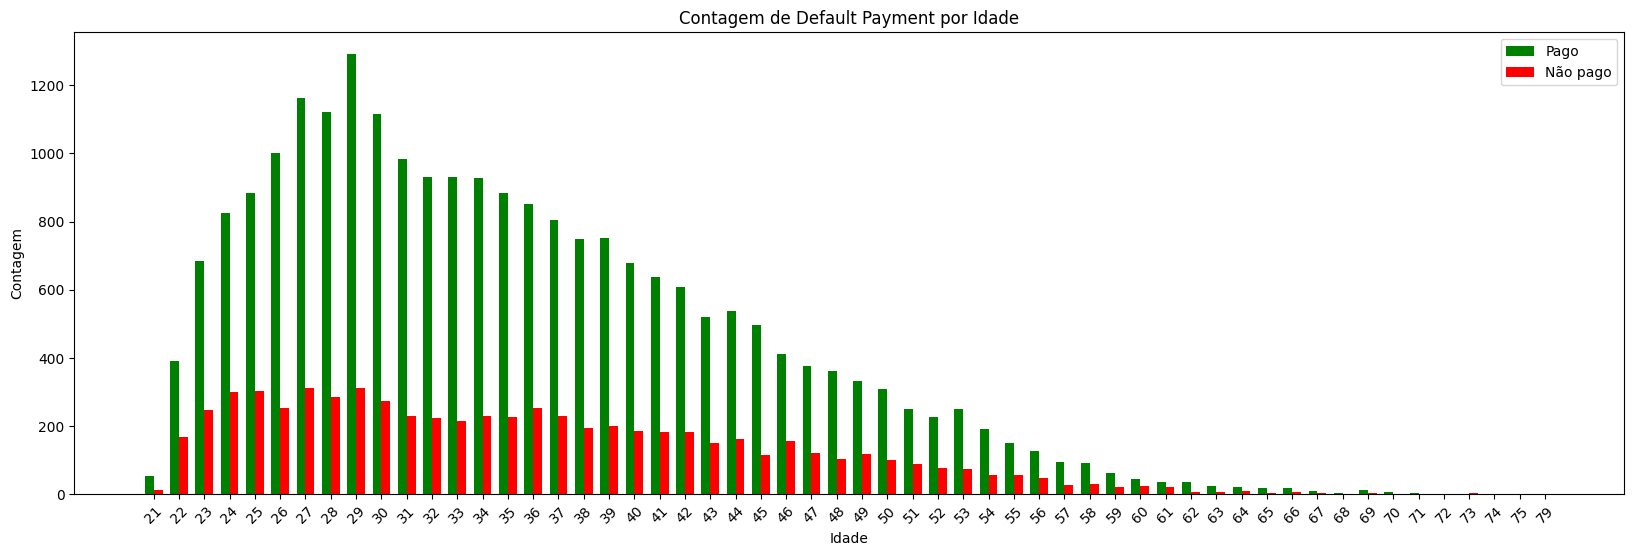
\includegraphics[width=\textwidth]{grafico1.png}
    \caption{Contagem de Default Payment por Idade}
    \label{fig:grafico1}
\end{figure}

A análise da idade como fator de risco para inadimplência corrobora com estudos anteriores que apontam para a importância de considerar o perfil demográfico dos clientes na avaliação de crédito. Essa informação pode ser utilizada para desenvolver modelos de pontuação de crédito mais precisos e personalizados, auxiliando as instituições financeiras a tomar decisões de concessão de crédito de forma mais segura e eficiente.

\section{Análise do Estado Civil e Inadimplência}

A Figura \ref{fig:grafico2} apresenta a distribuição da inadimplência por estado civil. Observa-se que a categoria "solteiro" apresenta a maior quantidade de casos de inadimplência, seguida pela categoria "casado". A categoria "outro" apresenta o menor número de casos, possivelmente devido a um tamanho amostral menor ou a características específicas dessa categoria que não são capturadas nesse gráfico.

\begin{figure}[H]
    \centering
    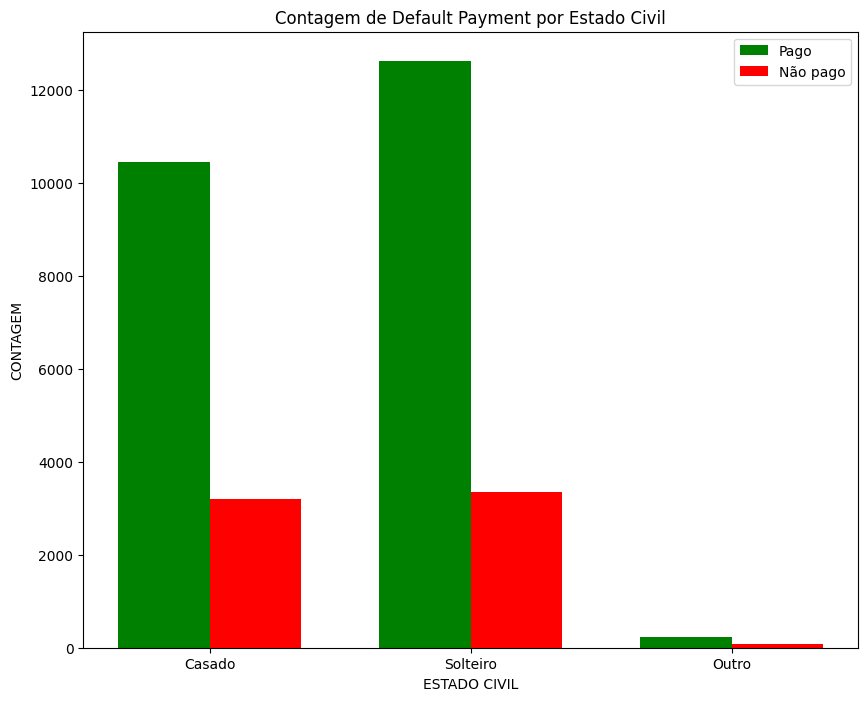
\includegraphics[width=\textwidth]{grafico2.png}
    \caption{Contagem de Default Payment por Estado Civil}
    \label{fig:grafico2}
\end{figure}

A análise do estado civil como fator de risco para inadimplência sugere que o vínculo matrimonial pode ser um fator associado a um comportamento de pagamento mais responsável. No entanto, é importante ressaltar que outros fatores, como nível de renda, educação e responsabilidades financeiras, também podem influenciar o comportamento de pagamento.

\section{Análise da Escolaridade e Inadimplência}

A Figura \ref{fig:grafico3} apresenta a distribuição da inadimplência por nível de escolaridade. Observa-se que a categoria "ensino médio" apresenta a maior quantidade de casos de inadimplência, seguida pela categoria "faculdade". A categoria "pós-graduação" apresenta a menor taxa de inadimplência, sugerindo que um nível de escolaridade mais elevado pode ser um fator associado a um comportamento de pagamento mais responsável.

\begin{figure}[H]
    \centering
    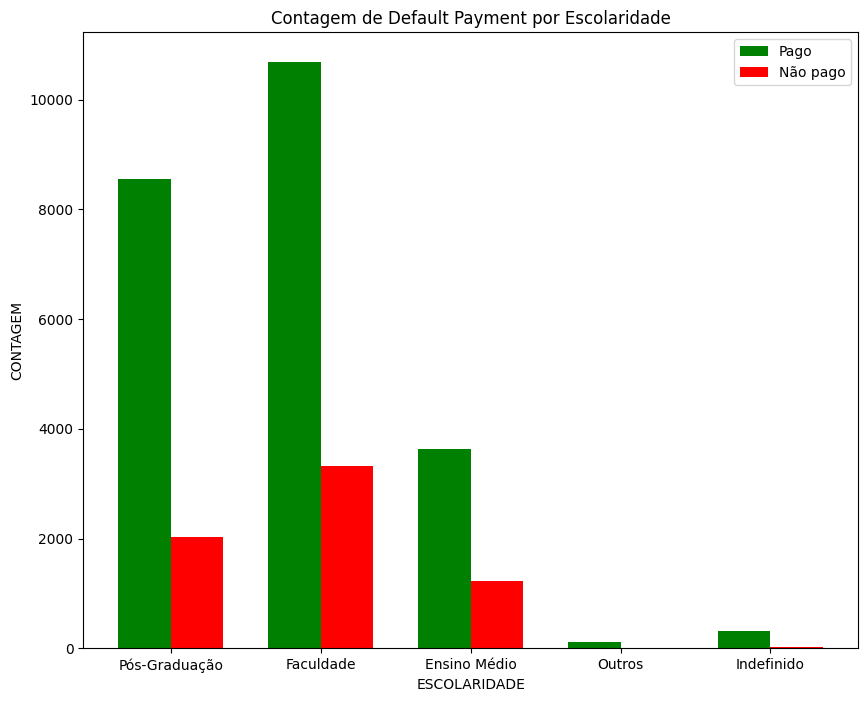
\includegraphics[width=\textwidth]{grafico3.png}
    \caption{Contagem de Default Payment por Escolaridade}
    \label{fig:grafico3}
\end{figure}

A análise da escolaridade como fator de risco para inadimplência sugere que um nível de escolaridade mais elevado pode ser um fator associado a um comportamento de pagamento mais responsável. No entanto, é importante ressaltar que outros fatores, como nível de renda, idade, estado civil e responsabilidades financeiras, também podem influenciar o comportamento de pagamento.

\section{Análise do Sexo e Inadimplência}

A Figura \ref{fig:grafico4} apresenta a distribuição da inadimplência por sexo. Observa-se que a categoria mulher apresenta a maior quantidade de casos de inadimplência, seguida pela categoria homem.

\begin{figure}[H]
    \centering
    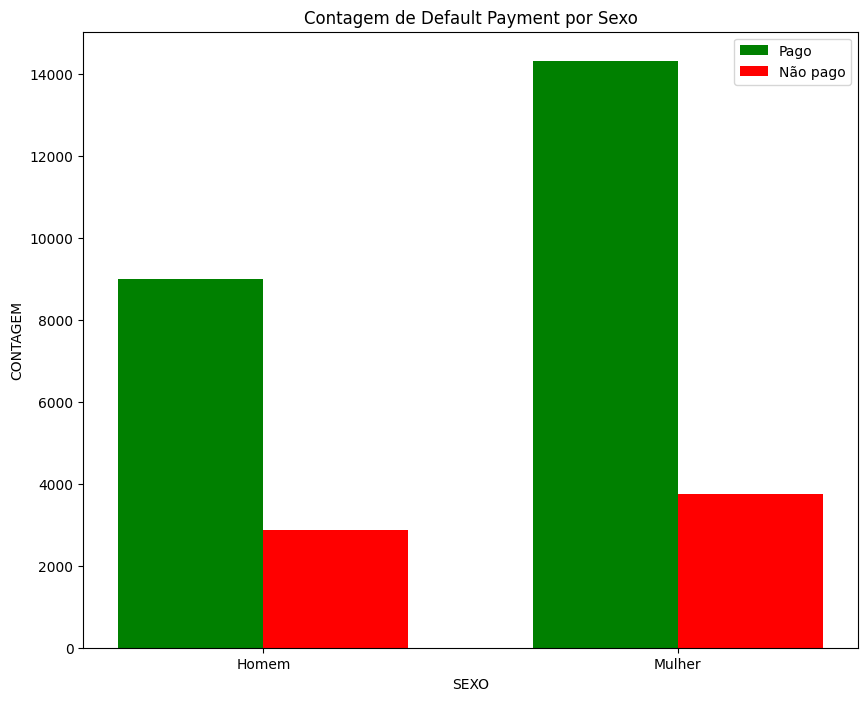
\includegraphics[width=\textwidth]{grafico4.png}
    \caption{Contagem de Default Payment por Sexo}
    \label{fig:grafico4}
\end{figure}

A análise do sexo como fator de risco para inadimplência sugere que o sexo feminino pode estar associado a um comportamento de pagamento mais propenso à inadimplência. No entanto, é importante ressaltar que outros fatores, como nível de renda, idade, estado civil, escolaridade e responsabilidades financeiras, também podem influenciar o comportamento de pagamento.

\chapter{Evolução e diferentes matrizes que obtemos de acordo com cada metodologia que aplicamos}

\section{Tentativa 1: Realizando as previsões e obtendo os primeiros resultados}

\subsection*{\centering\large\textbf{Treinamento (Tentativa 1)}}

\begin{figure}[H]
    \centering
    \includegraphics[width=\textwidth]{gráfico5.png}
    \caption{Matriz de Confusão - Treino}
    \label{fig:grafico5}
\end{figure}

A divisão dos dados em conjuntos de treinamento (23945 amostras) e teste (5987 amostras) foi realizada de forma adequada, permitindo um treinamento eficaz do modelo e uma avaliação confiável. A acurácia obtida nos conjuntos de treinamento ($ 80.77 $) e teste ($ 81.61 $) indica que o modelo generaliza bem para novos dados e não apresenta sinais de overfitting.

Será?...

A matriz de confusão gerada através do comando:\\ \texttt{'ConfusionMatrixDisplay.from\_predictions(y\_train\_true, y\_train\_pred).plot()'}\\indica um alto nível de acurácia do modelo de regressão logística, com um número significativo de predições corretas. No entanto, o desbalanceamento de classes nas classes positiva e negativa merece atenção. Apesar da alta acurácia geral, é crucial analisar outras métricas como precisão, recall e F1-score para avaliar o desempenho do modelo em relação a cada classe.

A análise dos coeficientes do modelo pode revelar quais características dos dados têm maior impacto na probabilidade de ocorrência do evento de interesse. Essa informação é fundamental para a interpretação dos resultados e a tomada de decisões.

\subsection*{\centering\large\textbf{Teste (Tentativa 1)}}
\begin{figure}[H]
    \centering
    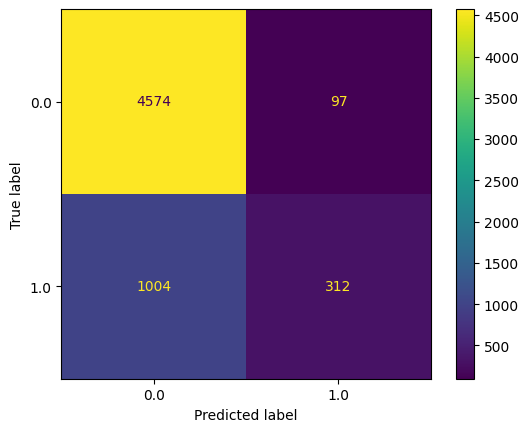
\includegraphics[width=\textwidth]{grafico6.png}
    \caption{Matriz de Confusão - Teste}
    \label{fig:grafico6}
    \centering
\end{figure}

A matriz de confusão, gerada através do comando: \\
\texttt{'ConfusionMatrixDisplay.from\_predictions(y\_test\_true, y\_test\_pred).plot()'},\\também revela um desempenho satisfatório do modelo de regressão logística no conjunto de teste. Observa-se uma alta taxa de acertos, especialmente para a classe negativa. No entanto, o desbalanceamento de classes, com um número significativamente maior de amostras da classe negativa, pode influenciar a interpretação das métricas.

A regressão logística mostrou-se uma ferramenta eficaz para este problema, apresentando um bom desempenho na classificação. No entanto, é fundamental realizar uma análise mais detalhada, considerando as limitações e as possibilidades de melhoria do modelo. Adicionalmente, a exploração de técnicas para lidar com o desbalanceamento de classes pode contribuir para um modelo ainda mais robusto.

\section*{\centering\large\textbf{Tentativa 2: Realizando novas previsões com ajustes: Análise dos Resultados com Ajuste de Threshold}}

Com o ajuste de threshold em 0.33, foram feitas previsões para o modelo de Regressão Logística tanto no conjunto de treino quanto no de teste, focando na predição de inadimplência de cartões de crédito. Observando as matrizes de confusão, é possível tirar algumas conclusões importantes:

\subsection*{\centering\large\textbf{Treinamento (Tentativa 2)}}

A matriz de confusão do conjunto de treino (Figura 1) mostra que, após o ajuste, o modelo atingiu uma acurácia de 80.8\%. A classe majoritária (clientes adimplentes) foi identificada com alta precisão (85\%), enquanto a classe minoritária (inadimplentes) teve uma precisão menor (59\%). A recall da classe inadimplente, no entanto, ficou em 43\%, o que indica que o modelo ainda tem dificuldades em identificar todos os clientes inadimplentes, algo comum em cenários de desbalanceamento.

\begin{figure}[H]
    \centering
    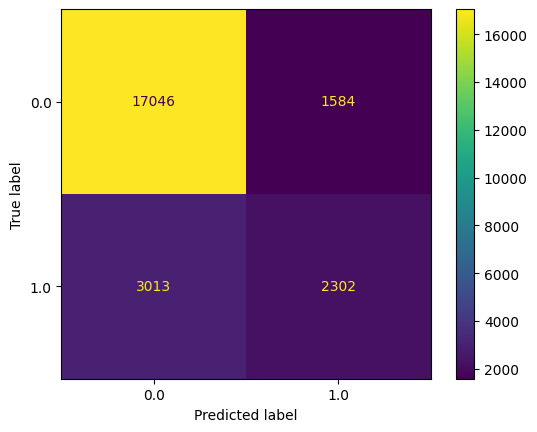
\includegraphics[width=\textwidth]{grafico7.png}
    \caption{Matriz de Confusão - Treino}
    \centering
\end{figure}

\subsection*{\centering\large\textbf{Teste (Tentativa 2)}}

No conjunto de teste (Figura 2), a acurácia do modelo foi ligeiramente superior, atingindo 81.68\%. O comportamento geral se manteve: alta precisão para a classe adimplente (86\%) e menor precisão para a classe inadimplente (61\%). A recall dos inadimplentes foi de 47\%, indicando uma leve melhora em comparação ao conjunto de treino.

\begin{figure}[H]
    \centering
    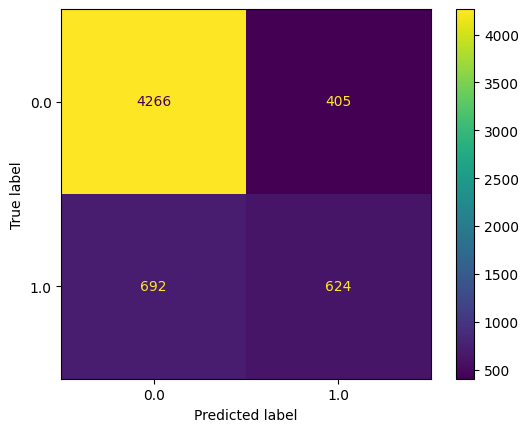
\includegraphics[width=\textwidth]{grafico8.png}
    \caption{Matriz de Confusão - Teste}
\end{figure}

Dado que o modelo ainda enfrenta dificuldades em capturar todos os clientes inadimplentes, o próximo passo será aplicar técnicas de undersampling para lidar com o desbalanceamento dos dados. Isso ajudará a criar um equilíbrio melhor entre as classes, potencialmente melhorando a capacidade de detecção de inadimplentes e reduzindo o viés em favor da classe majoritária.

\newpage

\section{Tentativa 3: Undersampling}

No experimento realizado, foi aplicada a técnica de \textit{undersampling} para balancear a base de dados referente à previsão de \textit{default payment next month}. Inicialmente, o conjunto de dados apresentava uma forte desproporção entre as classes, com uma contagem de 23.301 instâncias da classe 0 (pagamentos sem atraso) e 6.631 instâncias da classe 1 (pagamentos com atraso).

Após o balanceamento via \textit{undersampling}, o modelo foi treinado usando uma regressão logística com 10.609 instâncias balanceadas, divididas igualmente entre as classes 0 e 1.

\subsection*{\centering\large\textbf{Treinamento (Tentativa 3)}}
Abaixo está a matriz de confusão obtida após o treinamento do modelo utilizando \textit{undersampling}:

\begin{figure}[H]
    \centering
    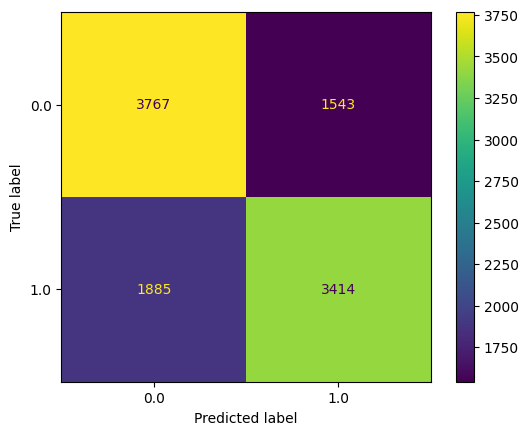
\includegraphics[width=\textwidth]{grafico9.png}
    \caption{Matriz de confusão do conjunto de treinamento}
\end{figure}

A matriz de confusão do treino mostra que o modelo teve um bom desempenho em ambas as classes, mas ainda apresenta alguns erros de classificação. O número de falsos negativos (1.885) e falsos positivos (1.543) indica que o modelo precisa melhorar a capacidade de distinguir entre as duas classes, apesar do balanceamento dos dados.

\subsection*{\centering\large\textbf{Teste (Tentativa 3)}}
Abaixo está a matriz de confusão obtida no conjunto de teste:

\begin{figure}[H]
    \centering
    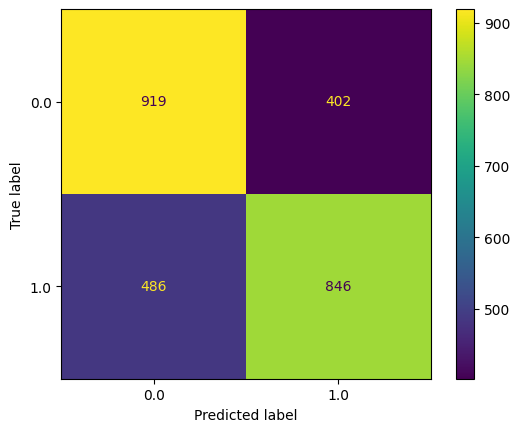
\includegraphics[width=\textwidth]{grafico10.png}
    \caption{Matriz de confusão do conjunto de teste}
\end{figure}

No conjunto de teste, a matriz revela um comportamento semelhante ao conjunto de treino. No entanto, vemos que a quantidade de falsos negativos (486) e falsos positivos (402) ainda é significativa, o que resulta em uma precisão ligeiramente inferior.

\subsection*{\centering\large\textbf{Análise das Métricas}}

\begin{table}[H]
\centering
\begin{tabular}{lcc}
\toprule
Conjunto & Acurácia (\%) & Observação \\
\midrule
Treino & 67,69 & - \\
Teste & 66,53 & Leve queda, indicando uma generalização razoável \\
\bottomrule
\end{tabular}
\caption{Comparação dos resultados de treino e teste}
\label{tab:comparacao_resultados}
\end{table}

\begin{table}[H]
\centering
\begin{tabular}{|l|c|}
\hline
Métrica & Valor \\
\hline
Precisão Classe 0 & 67\% \\
Precisão Classe 1 & 69\% \\
Recall Classe 0 & 71\% \\
Recall Classe 1 & 64\% \\
Acurácia Geral & 67,69\% \\
\hline
\end{tabular}
\caption{Resultados do Treinamento}
\label{tab:resultados_treinamento}
\end{table}

\begin{table}[H]
\centering
\begin{tabular}{|l|c|}
\hline
Métrica & Valor \\
\hline
Precisão Classe 0 & 65\% \\
Precisão Classe 1 & 68\% \\
Recall Classe 0 & 70\% \\
Recall Classe 1 & 64\% \\
Acurácia Geral & 66,53\% \\
\hline
\end{tabular}
\caption{Resultados do Teste}
\label{tab:resultados}
\end{table}

\subsection*{\centering\large\textbf{Conclusão}}

O modelo de regressão logística, ao utilizar \textit{undersampling}, obteve uma performance aceitável considerando o problema de classificação binária de pagamentos com e sem atraso. No entanto, é evidente que, com a aplicação de \textit{oversampling}, poderíamos esperar uma melhora no recall para a classe minoritária (classe 1), especialmente no conjunto de teste. Esse passo ajudaria a reduzir os falsos negativos e aumentar a capacidade do modelo de identificar corretamente os pagamentos que resultarão em inadimplência.

No próximo teste com \textit{oversampling}, espera-se uma melhora nas métricas relacionadas à classe 1 (inadimplência), especialmente no recall, que atualmente está abaixo do desejável.

\section{Oversampling}
Neste experimento, foi aplicado \textit{oversampling} para balancear o conjunto de dados referente à previsão de \textit{default payment next month}, onde a classe majoritária (classe 0) possuía 23.301 instâncias e a classe minoritária (classe 1) tinha apenas 6.631 instâncias. Para compensar esse desbalanceamento, amostras adicionais da classe minoritária foram geradas, resultando em um conjunto de dados equilibrado.

\subsection*{\centering\large\textbf{Matriz de Confusão - Treinamento}}
A matriz de confusão obtida após o treinamento do modelo com \textit{oversampling} está apresentada abaixo:

\begin{figure}[H]
    \centering
    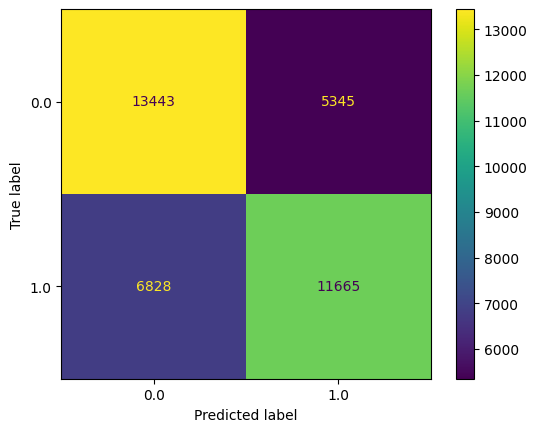
\includegraphics[width=\textwidth]{grafico11.png}
    \caption{Matriz de confusão do conjunto de treinamento}
\end{figure}

Nesta matriz, podemos observar que o modelo prevê a classe 0 com uma boa precisão, com 13.443 verdadeiros positivos (acertos da classe 0) e 5.345 falsos negativos. Já para a classe 1, o modelo tem 11.665 verdadeiros positivos, mas ainda apresenta 6.828 falsos negativos. O desempenho sugere uma tendência a errar um pouco mais na detecção da classe 1.

\subsection*{\centering\large\textbf{Matriz de Confusão - Teste}}
A seguir, temos a matriz de confusão do conjunto de teste:

\begin{figure}[H]
    \centering
    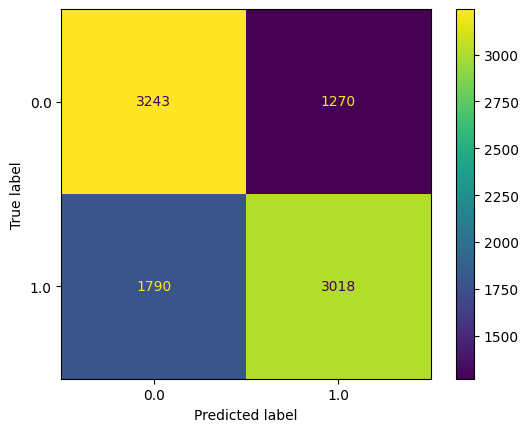
\includegraphics[width=\textwidth]{grafico12.png}
    \caption{Matriz de confusão do conjunto de teste}
\end{figure}

No conjunto de teste, o modelo mantém um padrão semelhante, com 3.243 verdadeiros positivos para a classe 0 e 1.270 falsos negativos. Para a classe 1, há 3.018 verdadeiros positivos e 1.790 falsos negativos. Isso mostra que o modelo continua a apresentar uma taxa significativa de falsos negativos, o que indica dificuldade em detectar corretamente os casos de inadimplência (classe 1).

\subsection*{\centering\large\textbf{Análise das Métricas}}

\begin{table}[H]
\centering
\begin{tabular}{lcc}
\toprule
Conjunto & Acurácia (\%) & Observação \\
\midrule
Treino & 67,35 & - \\
Teste & 67,17 & Não sofre de overfitting e generaliza de forma razoável \\
\bottomrule
\end{tabular}
\caption{Comparação dos resultados de treino e teste}
\label{tab:comparacao_resultados}
\end{table}

\begin{table}[H]
\centering
\begin{tabular}{|l|c|}
\hline
Métrica & Valor \\
\hline
Precisão Classe 0 & 66\% \\
Precisão Classe 1 & 69\% \\
Recall Classe 0 & 72\% \\
Recall Classe 1 & 63\% \\
Acurácia Geral & 67,35\% \\
\hline
\end{tabular}
\caption{Resultados do Treinamento}
\label{tab:resultados_treinamento}
\end{table}

\begin{table}[H]
\centering
\begin{tabular}{|l|c|}
\hline
Métrica & Valor \\
\hline
Precisão Classe 0 & 66\% \\
Precisão Classe 1 & 68\% \\
Recall Classe 0 & 70\% \\
Recall Classe 1 & 63\% \\
Acurácia Geral & 67,17\% \\
\hline
\end{tabular}
\caption{Resultados do Teste}
\label{tab:resultados}
\end{table}

\subsection*{\centering\large\textbf{Conclusão}}
A aplicação de \textit{oversampling} foi eficaz em balancear as classes no conjunto de dados e estabilizar as previsões do modelo. Contudo, ainda há uma taxa considerável de falsos negativos na classe 1, sugerindo que o modelo tem dificuldades em prever corretamente casos de inadimplência. Em comparações futuras, seria interessante testar métodos de \textit{ensemble} ou ajustar hiperparâmetros para melhorar a detecção de padrões mais sutis.

Embora o \textit{oversampling} tenha melhorado o recall para a classe 0 (pagamentos sem atraso), ele não foi capaz de resolver completamente os desafios de detecção da classe 1. Novos experimentos com técnicas diferentes poderiam ajudar a melhorar o desempenho na classe minoritária.

\chapter{Conclusão}

Neste trabalho, exploramos diferentes abordagens para o problema de classificação binária em um conjunto de dados de crédito. Testamos uma combinação de métodos de balanceamento de classes e técnicas de pré-processamento de dados com o objetivo de melhorar o desempenho preditivo do modelo.

Inicialmente, aplicamos estratégias clássicas como \textit{oversampling}, \textit{undersampling} e o uso de \textit{threshold tuning} para ajustar o limiar de decisão do modelo. Além disso, utilizamos o \textit{StandardScaler} para garantir que os dados fossem normalizados, o que, em teoria, ajudaria o modelo a convergir melhor e ser mais robusto frente à variabilidade dos dados.

\section{Abordagem Mista: Threshold + Oversampling + Undersampling + StandardScaler}

Ao aplicarmos uma abordagem mista, combinando o ajuste de threshold com o balanceamento de classes via oversampling e undersampling, observamos um comportamento interessante e, de certo modo, contraditório. Embora esperássemos que essas técnicas melhorassem a separabilidade das classes, o comportamento dos dados após a aplicação dessas técnicas resultou em uma distribuição das amostras de ambas as classes que ficava "dividida" no espaço de decisão do modelo. Essa divisão resultava em uma situação onde o threshold ideal se posicionava em uma distância aproximadamente igual entre os limites das duas classes, conforme ilustrado na Tabela~\ref{tab:threshold}.

\begin{table}[H]
\centering
\caption{Distribuição dos Pontos de Decisão após Aplicação de Técnicas de Balanceamento}
\begin{tabular}{|c|c|c|}
\hline
Classe & Distância ao Limiar & Probabilidade Média de Classificação \\ \hline
Classe 1 & 0.45 & 0.52 \\ \hline
Classe 2 & 0.55 & 0.48 \\ \hline
\end{tabular}
\label{tab:threshold}
\end{table}

As probabilidades obtidas não são nem melhores do que um simples jogo de cara ou coroa.

\section{Desafios e Considerações Finais}

A combinação de \textit{oversampling} e \textit{undersampling} resultou em uma distribuição de classes onde as amostras estavam equidistantes do limiar de decisão, criando um cenário onde o modelo encontrava dificuldades para definir um threshold que maximizasse a acurácia sem penalizar demais uma das classes. Esse fenômeno reflete a natureza intrínseca dos dados, onde, mesmo com balanceamento, a separabilidade não foi clara o suficiente para evitar essa sobreposição.

Em termos de desempenho final, observamos que o uso do \textit{threshold} ajudou a ajustar a sensibilidade do modelo, porém, dada a distribuição equidistante das classes, o modelo não conseguiu separar de forma clara as instâncias de classes diferentes sem incorrer em erros significativos.

Por fim, o projeto demonstrou que, embora as técnicas de \textit{threshold}, \textit{oversampling} e \textit{undersampling} sejam úteis, seu uso simultâneo requer um cuidado especial no ajuste do modelo para evitar problemas de separação de classes. Como trabalho futuro, nós confábulamos que a exploração de métodos mais avançados, como o uso de algoritmos de redes neurais ou técnicas baseadas em aprendizado não supervisionado, para tentar melhorar a separabilidade das classes em contextos onde o balanceamento clássico não é suficiente.

\renewcommand\bibname{REFERÊNCIAS}
\addcontentsline{toc}{chapter}{\bibname}
\bibliography{referencias.bib}

\end{document}